% -------------------------------------------------
% Capítulo: Implementación
% Orden del director (19-sep-2026): qué patrones de diseño se usaron, por qué y qué
% cambió; qué problemas hubo; cómo se creó la infraestructura y cómo se desplegó.
% Referencias archivo:línea verificadas contra el repositorio el 25-sep-2026.
% -------------------------------------------------

Este capítulo describe cómo se construyó Pymetory: la organización del código, los patrones de diseño aplicados y las razones de cada uno, los problemas reales que aparecieron durante el desarrollo y cómo se resolvieron, la infraestructura en la que corre el sistema y el proceso de despliegue. La forma de gestionar las tareas del proyecto se presenta aparte, en el Capítulo \ref{chap:gestion}.

\section{Organización del código}
\label{sec:imp_organizacion}

El repositorio sigue la estructura estándar de Laravel, con el frontend en React dentro de \texttt{resources/js}. La Tabla \ref{tab:imp_organizacion} resume sus partes principales.

\begin{table}[!htbp]
\centering
\caption{Organización del código fuente de Pymetory.}
\label{tab:imp_organizacion}
\begin{tabular}{|p{4.4cm}|c|p{8cm}|}
\hline
\textbf{Carpeta} & \textbf{Archivos} & \textbf{Contenido} \\
\hline
\texttt{app/Http/Controllers} & 24 & Controladores: inventario, consumo FEFO, transferencias, reportes, etiquetas, escáner, asistente, usuarios, ajustes, entre otros. \\ \hline
\texttt{app/Models} & 15 & Modelos Eloquent (\texttt{Material}, \texttt{Lote}, \texttt{Movimiento}, \texttt{Bodega}, \ldots). \\ \hline
\texttt{app/Console/Commands} & 3 & Revisiones programadas de alertas FEFO y de stock bajo, y el evaluador del asistente (\texttt{rag:evaluar}). \\ \hline
\texttt{app/Services} & 2 & Envío de alertas y proyección de reabastecimiento (\texttt{ProyeccionInventario}). \\ \hline
\texttt{database/migrations} & 32 & Definición versionada del esquema de la base de datos. \\ \hline
\texttt{resources/js/Pages} y \texttt{components} & 12 y 35 & Páginas Inertia y componentes React de la interfaz. \\ \hline
\texttt{tests} & 39 clases y 11 archivos & Pruebas PHPUnit y la suite Playwright (Capítulo \ref{chap:pruebas}). \\ \hline
\end{tabular}
\end{table}

\section{Patrones de diseño}
\label{sec:imp_patrones}

Al construir sobre Laravel, Pymetory hereda patrones que el framework trae resueltos: Modelo-Vista-Controlador como organización general, Active Record a través de Eloquent, una cadena de \textit{middleware} para procesar cada petición y un contenedor de servicios para la inyección de dependencias. Reutilizar esas soluciones probadas es una decisión razonable, pero no dice mucho de las decisiones del autor. Por eso esta sección se concentra en cinco lugares del código donde existía una alternativa legítima y se eligió conscientemente un patrón \cite{fowler2002poeaa}. Para cada uno se indica la alternativa descartada, la razón de la elección y lo que cambió en el sistema.

\subsection{Strategy: proveedores del asistente y canales de alerta}

\textbf{Qué es.} Una familia de algoritmos intercambiables entre los que se elige en tiempo de ejecución.

\textbf{Dónde está.} El \texttt{ChatLLMController} define un mapa de proveedores de modelo de lenguaje (Ollama local, OpenCode y cualquier API compatible con la de OpenAI; \texttt{app/Http/Controllers/ChatLLMController.php}, línea 369) y selecciona uno según la configuración del administrador. El mismo patrón aparece en \texttt{AlertService::send()} (\texttt{app/Services/AlertService.php}, línea 15), que decide por cuáles canales enviar una alerta.

\begin{lstlisting}[language=PHP]
// app/Services/AlertService.php (linea 15)
public function send(string $tipo, string $titulo, string $mensaje, ...): void
{
    $this->sendInApp($tipo, $titulo, $mensaje, $accionUrl, $icono);
    if (self::isActive('notif_telegram_activo')) { $this->sendTelegram(...); }
    if (self::isActive('notif_email_activo'))    { $this->sendEmail(...); }
}
\end{lstlisting}

\textbf{Alternativa descartada: Observer.} Observer es adecuado cuando un evento debe difundirse a todos los suscriptores. Aquí el problema es distinto: \emph{elegir} un proveedor o un canal según la configuración.

\textbf{Qué cambió.} Cambiar de proveedor de modelo de lenguaje es una modificación de configuración, no de código. Esto permitió pasar durante el proyecto de modelos locales a proveedores en la nube, y en la versión final dejar un modelo gratuito de Ollama Cloud como principal con un modelo local de respaldo, sin tocar el controlador.

\subsection{Chain of Responsibility: control de acceso}

\textbf{Qué es.} Una petición pasa por una serie de manejadores, cada uno con una única responsabilidad, que pueden detenerla.

\textbf{Dónde está.} Cada ruta declara su cadena: \texttt{auth} (sesión), \texttt{verified} y \texttt{role:admin}. El eslabón de rol es propio del proyecto (\texttt{app/Http/Middleware/CheckRole.php}, línea 19):

\begin{lstlisting}[language=PHP]
public function handle(Request $request, Closure $next, string $role): Response
{
    if (!$request->user() || $request->user()->role !== $role) {
        abort(403, 'No tienes permisos de ' . strtoupper($role) . ' ...');
    }
    return $next($request);
}
\end{lstlisting}

\textbf{Alternativa descartada: una verificación única en cada controlador.} Es válida con una sola regla de acceso, pero mezcla la seguridad con la lógica de negocio y obliga a repetirla.

\textbf{Qué cambió.} La política de acceso se lee en el archivo de rutas y se corrige en un solo lugar. Cuando en la revisión final se detectó que las rutas de usuarios y claves de API no exigían el rol de administrador, la corrección consistió en añadir \texttt{role:admin} al grupo de rutas (Sección \ref{sec:imp_problemas}).

\subsection{Active Record: reglas del lote en el propio modelo}

\textbf{Qué es.} Cada objeto representa una fila de la base de datos y contiene su persistencia y sus reglas de dominio.

\textbf{Dónde está.} El modelo \texttt{Lote} concentra las reglas que dependen de él: si está crítico por vencimiento (\texttt{getIsCriticalAttribute}, línea 80, con el umbral configurable leído en \texttt{diasCriticos()}), su valor (\texttt{getValorTotalAttribute}, línea 92) y el orden FEFO (\texttt{scopeFefoOrder}, línea 105), en \texttt{app/Models/Lote.php}.

\textbf{Alternativa descartada: Repository o Data Mapper.} Son útiles cuando se necesita independencia del motor de persistencia o hay varias fuentes de datos. Pymetory usa un solo motor (MySQL), y una capa Repository sobre Eloquent solo reenviaría llamadas.

\textbf{Qué cambió.} La regla de criticidad vive en un solo lugar. Cuando se descubrió que el tablero ignoraba el umbral configurado por el administrador, bastó con cambiar el modelo para que tablero, inventario y alertas quedaran coherentes.

\subsection{Transaction Script: despacho FEFO}

\textbf{Qué es.} La lógica de una operación de negocio se organiza como un procedimiento único que la atiende de principio a fin.

\textbf{Dónde está.} \texttt{ConsumptionController::store()} (\texttt{app/Http/Controllers/ConsumptionController.php}, línea 37) ordena los lotes activos por vencimiento, descuenta la cantidad pedida lote por lote, marca como consumidos los que se agotan y registra cada salida en el Kardex, todo dentro de una transacción:

\begin{lstlisting}[language=PHP]
DB::transaction(function () use ($material, $quantityToConsume, $validated) {
    $lotes = Lote::where('material_id', $material->id)
        ->where('status', 'active')->orderBy('expiration_date', 'asc')->get();
    $remaining = $quantityToConsume;
    foreach ($lotes as $lote) {
        if ($remaining <= 0) break;
        $consumption = min($lote->quantity, $remaining);
        $lote->quantity -= $consumption;
        if ($lote->quantity <= 0) { $lote->status = 'consumed'; }
        $lote->save();
        Movimiento::create([ /* lote, usuario, salida, cantidad, motivo */ ]);
        $remaining -= $consumption;
    }
});
\end{lstlisting}

\textbf{Alternativa descartada: Domain Model.} Un modelo de dominio rico conviene cuando las reglas son numerosas e interdependientes. El despacho FEFO es un procedimiento lineal de unas treinta líneas.

\textbf{Qué cambió.} La transacción garantiza que un despacho que toca varios lotes quede completo o no quede: si falla a mitad, ni los lotes ni el Kardex cambian.

\subsection{Factory Method: datos de prueba}

\textbf{Qué es.} La creación de objetos se delega a un componente especializado.

\textbf{Dónde está.} Las \textit{factories} de \texttt{database/factories} construyen materiales, bodegas, lotes y usuarios válidos. Por ejemplo, \texttt{LoteFactory::definition()} (línea 14) crea un lote con su material y su bodega.

\textbf{Alternativa descartada: construir los objetos a mano en cada prueba.} Es aceptable con pocas pruebas y objetos simples. Aquí un lote depende de un material y una bodega, y las pruebas automatizadas son decenas.

\textbf{Qué cambió.} Las pruebas describen solo lo que les interesa (por ejemplo, un lote que vence en 20 días) y el resto de datos se completa de forma consistente.

\section{Proyección de reabastecimiento}
\label{sec:imp_proyeccion}

Los requerimientos RF-09 y RF-10 y el nivel de analítica predictiva del alcance se implementaron en el servicio \texttt{ProyeccionInventario}, que calcula todo a partir del Kardex, sin datos escritos en el código:

\begin{itemize}
    \item \textbf{Consumo diario.} Promedio móvil simple: lo que salió del insumo por producción, venta, desperdicio o escáner en los últimos 28 días, dividido entre 28. Las transferencias no cuentan porque el insumo solo cambia de bodega, y los ajustes tampoco, porque corrigen el conteo y no reflejan demanda.
    \item \textbf{Cobertura y agotamiento.} La existencia activa dividida entre el consumo diario da los días que alcanza; sumados a la fecha de hoy, la fecha probable de agotamiento.
    \item \textbf{Punto de reorden.} Consumo diario $\times$ días de entrega del proveedor + stock mínimo, según el modelo de punto de reorden descrito en la Sección \ref{sssec:eoq_rop}. Los días de entrega los registra el administrador por insumo; si no están, el sistema no inventa el punto de reorden y lo indica. Un insumo está por reponer cuando su existencia llega a ese punto o baja de su mínimo; si no, se muestra la última fecha para pedir a tiempo.
    \item \textbf{Diagnóstico.} Para explicar una variación, el servicio agrupa las entradas y salidas del insumo por motivo en los últimos días y las compara con el periodo anterior de igual duración.
\end{itemize}

El promedio móvil supone que el consumo de los próximos días será como el de las últimas semanas: no anticipa temporadas ni cambios bruscos, lo que se propone como trabajo futuro. La vista Reabastecimiento muestra estos valores y grafica el consumo por día, semana o mes, y el asistente los usa en dos intenciones nuevas (\texttt{forecast} y \texttt{consumption}). Once pruebas PHPUnit verifican los cálculos con fechas fijas, la exclusión de transferencias y ajustes, y que la clasificación de las 106 preguntas de las baterías de evaluación no cambió.

\section{Problemas enfrentados y cómo se resolvieron}
\label{sec:imp_problemas}

La Tabla \ref{tab:imp_problemas} reúne los problemas más significativos del desarrollo. Cada uno tiene como evidencia el commit que lo corrigió en el repositorio.

{\small
\begin{longtable}{|p{3.6cm}|p{5.6cm}|p{4.2cm}|p{1.4cm}|}
\caption{Problemas del desarrollo y su solución.}
\label{tab:imp_problemas}\\
\hline
\textbf{Problema} & \textbf{Causa} & \textbf{Solución} & \textbf{Commit} \\
\hline
\endfirsthead
\hline
\textbf{Problema} & \textbf{Causa} & \textbf{Solución} & \textbf{Commit} \\
\hline
\endhead
El despliegue automático fallaba al actualizar el código en el servidor. & El repositorio del servidor usaba HTTPS sin credenciales y \texttt{git pull} pedía usuario. & El flujo de despliegue se autentica con un token efímero de cada ejecución. & \texttt{91732b6} \\ \hline
La compilación del frontend fallaba en integración continua. & Un archivo importado por la aplicación (\texttt{theme.ts}) no estaba versionado. & Se agregó el archivo al repositorio. & \texttt{90da6f5} \\ \hline
El asistente devolvía respuestas vacías con modelos que razonan antes de responder. & El razonamiento consumía todo el límite de tokens y dejaba vacío el contenido. & Se filtra el razonamiento y se reintenta con un límite mayor. & \texttt{1c9e162} \\ \hline
El asistente respondía con ``la lista completa'' del inventario. & Las expresiones regulares no soportaban tildes (UTF-8) y un material inexistente devolvía lotes de otros materiales. & Clasificación compatible con UTF-8 y respuesta explícita de ``material no registrado''. & \texttt{5c7c2ef} \\ \hline
Cualquier visitante podía registrarse como administrador. & El registro público aceptaba el rol enviado en la petición; además, las rutas de usuarios y claves no exigían el rol. & El registro creó solo operarios y las rutas quedaron bajo \texttt{role:admin}; en la revisión final se eliminó el registro público. & \texttt{a802cbb}, \texttt{9d0efb8} \\ \hline
Se podía despachar un lote en cuarentena o vencido, y el despacho por lote o por QR no aplicaba FEFO. & Solo el despacho automático ordenaba por vencimiento; los demás no validaban estado ni fecha. & Una sola regla en el modelo \texttt{Lote} para todo despacho; un vencido solo se da de baja como desperdicio. & \texttt{9d0efb8} \\ \hline
Borrar un usuario eliminaba su historial del Kardex. & Las llaves foráneas de \texttt{movimientos} tenían borrado en cascada. & El modelo rechaza modificar o borrar movimientos y las llaves pasaron a \texttt{restrict}. & \texttt{f53a7d0} \\ \hline
El inicio de sesión fallaba en producción. & Detrás del túnel de Cloudflare, Laravel generaba redirecciones \texttt{http} bloqueadas por el navegador. & Se declararon los proxies de confianza (\texttt{trustProxies}). & \texttt{f174905} \\ \hline
El tablero mostraba tendencias que no provenían de datos. & Valores de maqueta que quedaron en el controlador. & Tendencias calculadas contra 30 días atrás y rotación desde el Kardex. & \texttt{361d0af} \\ \hline
El umbral de vencimiento configurado no se reflejaba en el tablero. & El tablero usaba 15 días fijos; solo alertas y reportes leían el ajuste. & El modelo \texttt{Lote} lee el umbral configurado. & \texttt{66456a3} \\ \hline
Textos invisibles en algunos temas visuales. & La capa de temas reasignaba colores de utilidades como \texttt{bg-white} sin ajustar el texto. & Tokens de color por tema en lugar de colores fijos. & \texttt{75f694d} \\ \hline
Al corregir un tema visual se descomponía otro. & Más de cien reglas reasignaban clases de color una por una, varias con \texttt{!important}, y competían entre sí. & Cada tema define sus tokens y redefine la paleta completa de Tailwind; se eliminaron las reglas por clase. & \texttt{10787fd} \\ \hline
La pantalla de alertas mostraba avisos de ejemplo. & La vista era una maqueta con textos fijos; las alertas reales se guardaban pero nadie las leía. & La vista consulta la tabla \texttt{notifications}; se agregaron marcado como leída y la no repetición de avisos. & \texttt{10787fd} \\ \hline
El formulario de transferencias no listaba lotes. & Los datos enviados a la vista no incluían la bodega ni el número de lote que el formulario filtraba. & Se agregaron esos campos a los datos del inventario. & \texttt{10787fd} \\ \hline
El asistente respondió que ningún lote vencía en la semana cuando sí había. & El contexto incluía lotes ya consumidos, con fechas pasadas, y no indicaba la fecha del día. & Solo lotes con existencias, ventana de días según la pregunta y fecha de hoy en el contexto; prueba de regresión. & \texttt{ec76a78} \\ \hline
Recibir una orden de compra creaba el lote con vencimiento de ``hoy más un año''. & La recepción no pedía los datos del lote: fecha, número y bodega se fijaban en el código. & La recepción exige número de lote, vencimiento y bodega por ítem; se agregó el ingreso de lotes para insumos ya registrados. & \texttt{2987679} \\ \hline
El pan terminado aparecía siempre como crítico y la ocupación sumaba kilos con unidades. & Un único umbral de 15 días para productos que duran de 5 a 7 días; capacidad sin unidad. & Umbral FEFO por insumo y unidad de capacidad por bodega; ocupación global como promedio. & \texttt{de53e61} \\ \hline
El asistente acertó 34 de 50 consultas en la primera medición. & Contextos sin costos, sin ajustes de conciliación ni totales; lotes no reconocidos por su número real. & Contextos completos y clasificador revisado; la misma batería pasó a 49 de 50. & \texttt{48f092f} \\ \hline
Seis tipos de incumplimiento de WCAG 2.1 AA. & Contraste bajo, botones de solo ícono sin nombre y campos sin etiqueta. & Acento sólido por tema, nombres accesibles y etiquetas; cero incumplimientos automáticos en el tema por defecto. & \texttt{fb0e9bb} \\ \hline
\end{longtable}
}

Además de los defectos de código, la operación del servidor mostró dos problemas de recursos. Dos procesos de un proyecto ajeno a la tesis, alojado en el mismo servidor, llevaban seis días ocupando dos de los cuatro núcleos, lo que hacía muy lentos los modelos de lenguaje locales; se detuvieron y ese proyecto se retiró del repositorio de la tesis. Y al evaluar modelos, cargar varios a la vez agotó la memoria y dejó la aplicación sin servicio unos seis minutos; desde entonces Ollama tiene un límite de 14~GB y un solo modelo cargado a la vez, de modo que no puede afectar a la base de datos ni a la aplicación.

\section{Infraestructura}
\label{sec:imp_infraestructura}

El sistema corre en una instancia de Oracle Cloud de la capa gratuita \textit{Always Free} \cite{oci_always_free}: procesador ARM de 4 núcleos, 24~GB de memoria y 200~GB de disco. La Figura \ref{fig:imp_despliegue} muestra sus componentes:

\begin{itemize}
    \item \textbf{Acceso.} El dominio \texttt{app.pymetory.com} se publica mediante un túnel de Cloudflare, que establece la conexión desde el servidor hacia Cloudflare. El servidor no expone puertos de la aplicación a internet y el certificado TLS lo gestiona Cloudflare.
    \item \textbf{Aplicación y datos.} Laravel 13 sobre PHP 8.3, con MySQL 8.0 en el mismo servidor, ejecutado por PHP-FPM detrás de Nginx, que además entrega directamente los archivos estáticos (JavaScript, estilos e imágenes). Al principio se usaba el servidor de desarrollo de PHP (\texttt{artisan serve}), que atiende una petición a la vez: una consulta lenta al asistente o las imágenes de la página de inicio dejaban esperando a las demás. El cambio redujo el tiempo de carga del inicio de sesión de varios segundos a unos 0,3 segundos.
    \item \textbf{Modelos de lenguaje.} El modelo principal es \texttt{gpt-oss:120b-cloud}, de la capa gratuita de Ollama Cloud. Si falla o responde vacío, contesta un modelo local de respaldo (\texttt{qwen3.5:9b}), y si ese también falla, el asistente muestra en modo texto los datos que recuperó de la base. En el servidor, el respaldo tardó 56~s con el modelo en frío y 33~s ya cargado, frente a cerca de un segundo del modelo en la nube; por eso es un respaldo y no el modelo principal. Ollama no puede usar más de 14~GB de memoria, y ante falta de memoria el sistema operativo lo detiene a él antes que a la base de datos o a la aplicación.
    \item \textbf{Ensayo de modelos locales.} En el servidor se midieron memoria y tiempo de los modelos locales que caben en ese límite (27 de septiembre de 2026). \texttt{gemma4:12b} y \texttt{qwen3.5:9b} cargaron su contexto máximo de 256\,000 tokens con unos 11,5~GB, pero leyeron a 7,5 y 13,9 tokens por segundo: unos 4\,100 tokens les tomaron 9 y 5 minutos. \texttt{qwen3:14b} no terminó de leerlos en 15 minutos. Sin GPU, entregar al modelo todo el inventario en cada pregunta no es viable; el diseño RAG, que le entrega solo unos cientos de tokens ya filtrados, es lo que permite responder en segundos.
    \item \textbf{Tareas programadas.} Un \textit{cron} ejecuta cada minuto el programador de Laravel, que revisa cada hora los lotes por vencer y el stock bajo.
    \item \textbf{Respaldos.} Cada noche se genera un volcado comprimido de la base de datos con \texttt{mysqldump}, y antes de cada cambio delicado ---como la migración que hizo inmutable el Kardex el 25 de septiembre de 2026--- se generó uno adicional. Todas las copias quedan en el mismo servidor (ver Trabajos Futuros).
\end{itemize}

\begin{figure}[H]
\centering
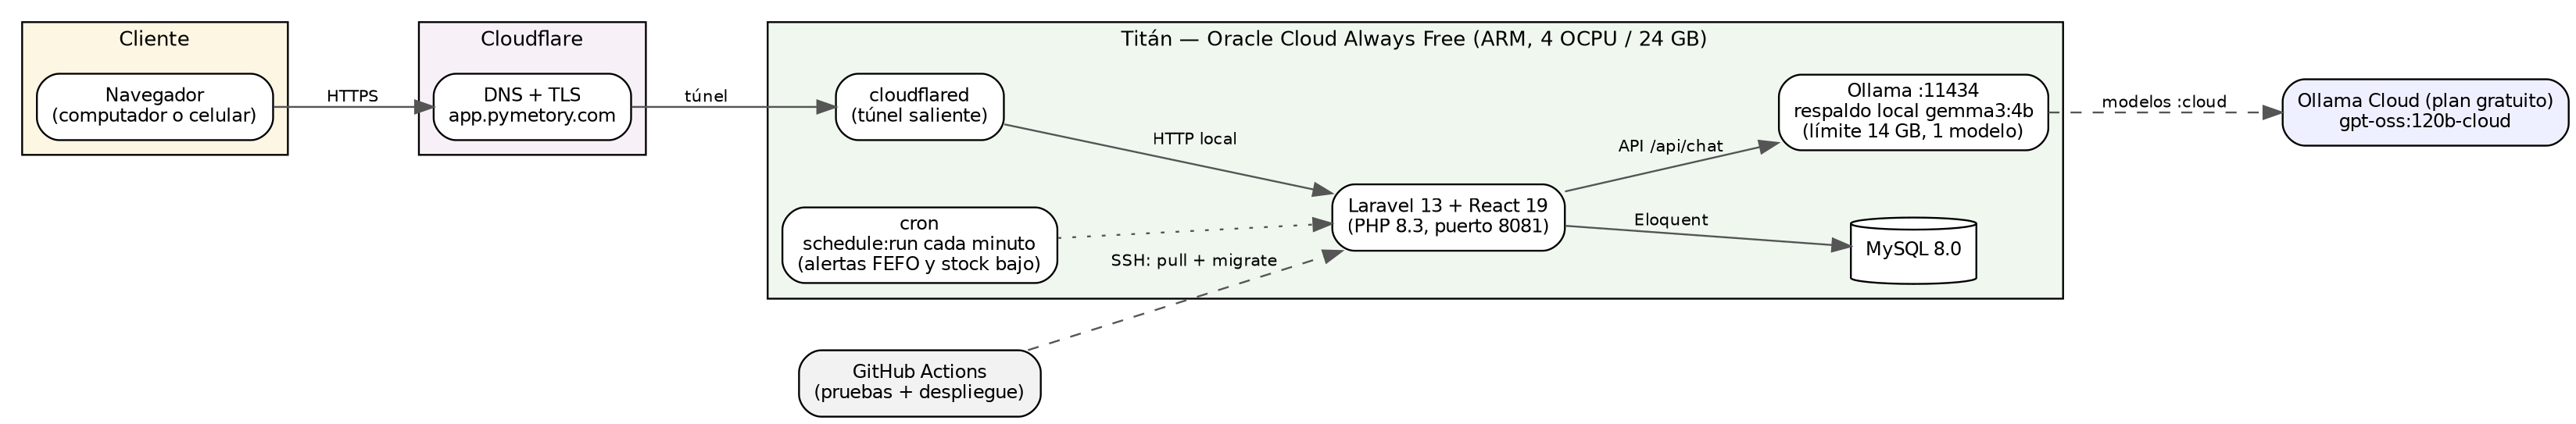
\includegraphics[width=0.9\textwidth]{Anexos/Imagenes/DiagramaDespliegue.png}
\caption{Infraestructura de producción de Pymetory.}
\label{fig:imp_despliegue}
\end{figure}

\section{Despliegue}
\label{sec:imp_despliegue}

El despliegue está automatizado con GitHub Actions (\texttt{.github/workflows/deploy.yml}). Cada cambio que llega a la rama principal recorre tres etapas:

\begin{enumerate}
    \item \textbf{Revisión.} Verificación de sintaxis de los archivos PHP.
    \item \textbf{Pruebas.} Instalación de dependencias, compilación del frontend y ejecución de la suite PHPUnit. Si una prueba falla, el despliegue no continúa.
    \item \textbf{Despliegue.} Conexión por SSH al servidor, actualización del código, instalación de dependencias de producción, migraciones, regeneración de cachés y reinicio del servicio; el frontend compilado desde el mismo commit se sube aparte. Producción usa \texttt{APP\_DEBUG=false}, para que un error no exponga detalles internos.
\end{enumerate}
